\documentclass[12pt,a4paper,ngerman]{article}
\usepackage{stylesheet}
\begin{document}
\TUHeader                          %  Bitte Ausfüllen!!!
%----------------------------
{Übung F: Übertragungsverhalten nachrichtentechnischer Systeme}                       %  Übungstitel
%----------------------------
{25.11.2014}                        %  Übungsdatum
%----------------------------
{05}                            %  Gruppen-Nr.
%----------------------------
{Thomas Neff}                   % Name des Protokollführers
%----------------------------
{
1.~Daniel Freßl, 1230028\\
2.~Thomas Neff, 1230319\\                    %  Übungsteilnehmer
3.~Thomas Pichler, 1230320 \\                   %  ...bei <4 Teilnehmer auskommentieren
4.~Martin Winter, 1130688\\
5.~Bernadette Schreyer, 1073076\\
}
%----------------------------
{Ao.Univ.-Prof. Dipl.-Ing. Dr. techn. Erich Leitgeb}
{Max Henkel}                          %  Betreuer
%----------------------------
{Graz}                              %  Ort der Protokollerstellung
{\today}                            %  Datum Protokollerstellung




\pagebreak
  
\tableofcontents
  
\pagebreak

%-------------------------------------------------------------------------------
%
% Beginn des Protokolls
%
%-------------------------------------------------------------------------------

\section*{Aufgabe 1}


\begin{framed}
\textbf{I$^2$C Anwendungsbeispiel}\\
Sie haben einen Controller gebaut, welcher die Funktion einer Wendeschützschaltung übernimmt. Der Controller verfügt neben für den "Inselbetrieb" notwendigen Eingängen über eine I$^2$C Schnittstelle. Diese Schnittstelle erlaubt es, zusätzliche Parameter einzustellen, beziehungsweise Betriebszustände (Fehlermeldungen) abzufragen. Erklären Sie
\begin{enumerate}
\item Wie sieht ihr Controller aus (Skizze mit Interface)?
\item Arbeitet er als Master oder Slave?
\item Erklären Sie die Register ihres Controllers bzw. deren Funktion?
\item Wie funktioniert die Steuerung des Controllers über I$^2$C Bus (Beispiel)?
\end{enumerate}
\end{framed}

\pagebreak
\section*{Aufgabe 2}


\begin{framed}
\textbf{I$^2$C Bus-Arbitrierung}\\
Zeigen Sie anhand vpn Beispielen wie die Arbitrierung am I$^2$C Bus für 2 Master funktioniert, wenn die Master Write-Befehle an Slaves schicken. Geben Sie für folgende Situationen jeweils ein Beispiel an:
\begin{enumerate}
\item unterschiedliche Zieladresse und unterschiedliche Daten
\item gleiche Zieladresse und unterschiedliche Daten
\item gleiche Zieladresse und gleiche Daten
\end{enumerate}
Zeigen Sie, welche Daten am Bus gesendet werden und wann sich welcher Master zurückzieht und begründen Sie dies.
\end{framed}

Arbitrierung von zwei oder mehreren Mastern auf dem I2C-Bus:\\
\\
Ein Master darf nur mit einer Übertragung starten wenn der Bus gerade frei ist.\\
Zwei oder mehrere Master können gleichzeitig starten wenn sie die Start-Condition innerhalb der minimum hold time senden.\\
Jeder Master kontrolliert bei jedem gesendeten Bit (während die SCL high ist) ob auf der SDA-Leitung der Pegel anliegt den er gesendet hat. Wenn ein anderer Pegel anliegt (nur bei gesendet HIGH aber auf SDA LOW möglich - wired-AND) beendet der Master sofort die Übertragung und der andere Master kann seine Übertragung weiter durchführen.\\
Die Arbitrierung kann den ganzen Sendevorgang dauern, wenn beide Master an die selbe Adresse die selben Daten senden.\\
\\
\begin{figure}[h!]
\begin{center}
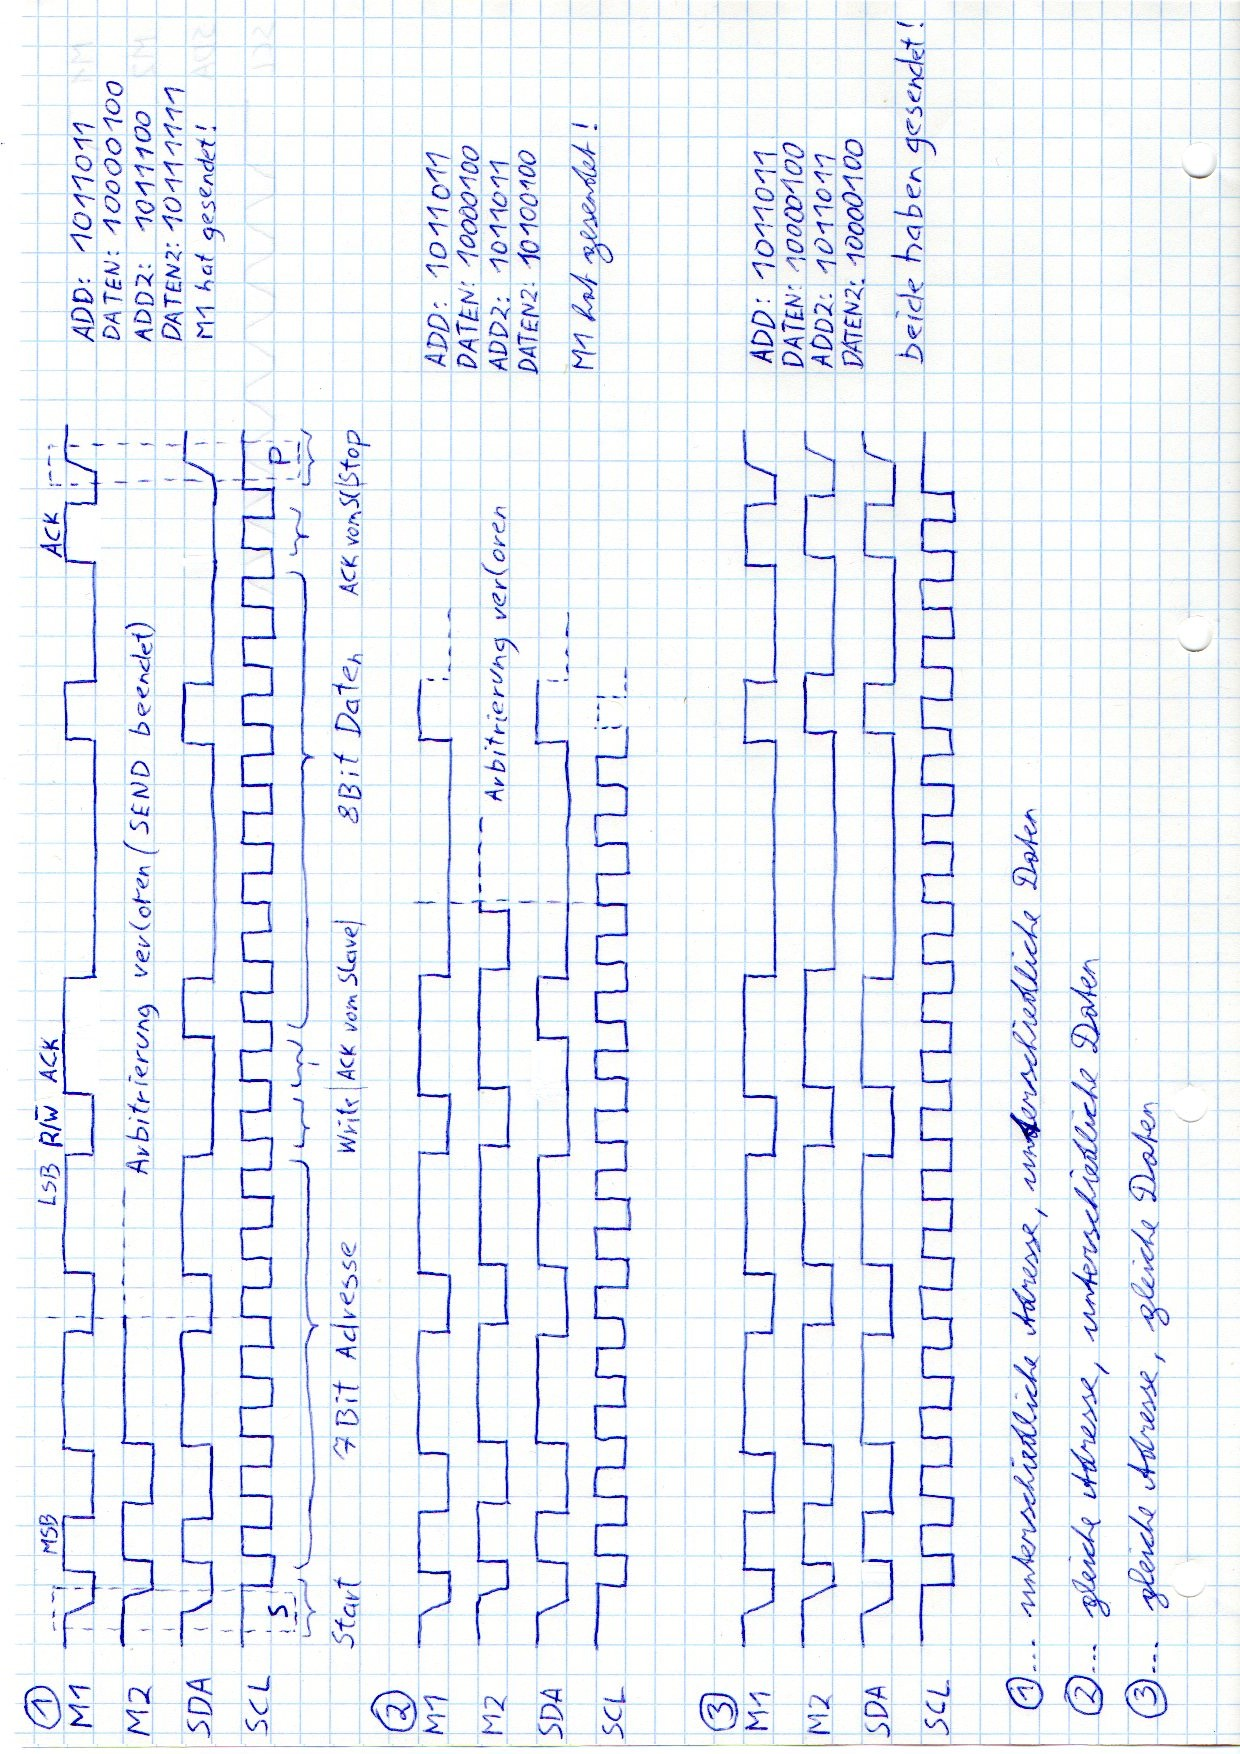
\includegraphics[scale=0.72]{figures/Aufgabe_3_2_arbitrierung.jpg} 
\caption{Arbitrierung}
\end{center}
\vspace{-20pt}
\end{figure}\\

\pagebreak

\section*{Aufgabe 3}


\begin{framed}
\textbf{I$^2$C-Bus vs. SPI-Bus}\\
Bussysteme spielen eine wichtige Rolle in eingebettenen Systemen. Ermitteln Sie deshalb bedeutende Kenngrößen zu deren Vergleich und identifizieren Sie dies sowohl für den I$^2$C- als auch für den SPI-Bus. \\
Beschreiben Sie zusätzlich die Zugriffsmethoden für obige Bussysteme und stellen Sie den Ablauf eine Buszyklus dar (Write und Read zwischen Master und Slave). Begründen Sie auch, ob obige Bussysteme mit mehreren Masterknoten verwendet werden können.
\end{framed}
\begin{table}[h!]
  \begin{center}
    \begin{tabular}{| l | p{6cm} | p{6cm} |}
    \hline
     Vergleichskriterium & I$^2$C & SPI  \\ \hline \hline
    Leitungen & 2 gemeinsame Leitungen \begin{itemize}
    \item SDA (Serial Data Line)
    \item SCL (Serial Clock Line) 
\end{itemize}     & 	3 gemeinsame Leitungen \begin{itemize}
    \item SCLK (serial clock) 
    \item MOSI (Master Output, Slave Input)
    \item MISO (Master Input, Slave Output)
    \end{itemize}
    1 individuelle Leitung pro Slave
    \begin{itemize}
    \item CS (Chip-Select)
    \end{itemize}
       \\ \hline
       Geschwindigkeit & $<400$kHz & $>1$MHz \\ \hline
       Protokollkomplexität & mittel & gering \\ \hline
       Chippreise & höher & niedriger \\ \hline
       Sendeverfahren & \textbf{halbduplex} (Daten können abwechselnd, aber nicht gleichzeitig, in beide Richtungen übertragen werden) & \textbf{vollduplex} (Daten können in beide Richtungen gleichzeitig übertragen werden \\ \hline
    \end{tabular}
  \end{center}
  \caption{Vergleichskriterien}
\end{table}
Der wesentliche Unterschied besteht darin, dass I$^2$C den Busverkehr über 2 Leitungen abhandelt, während SPI die Selektion über eine extra Chip-Select Leitung vornimmt. \\
\begin{figure}[h]
\begin{center}
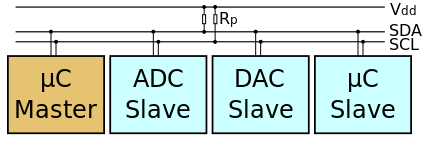
\includegraphics[scale=0.5]{figures/i2c.png} 
\caption{I$^2$C}
\end{center}
\vspace{-20pt}
\end{figure}\\
\textbf{I$^2$C} verwendet also 2 Leitungen mit 7-Bit Adressierung, jedes Device am Bus kann als Master oder Slave auftreten, es können auch mehrere Master und mehrere Slaves am gleichen Bus betrieben werden. \\
Ein typischer Sendevorgang sieht folgendermaßen aus: Der Master sendet sein Startbit, gefolgt von der 7-Bit Adresse des Slaves, mit welchem er kommunizieren möchte und einem Bit, ob ein \textbf{R}ead oder \textbf{W}rite Vorgang stattfinden soll. Ist dieser Slave an dieser Adresse am Bus vorhanden, so sendet er zuerst ein \textbf{ACK}(Acknowledge) für diese Adresse, woraufhin der Master in den gewünschten Modus wechselt und der Slave ebenso in den komplementären Modus wechselt (Read|Write oder Write|Read). \\
Möchte der Master schreiben, so sendet er ein Byte und der Slave sendet ACK, möchte er die Übertragung stoppen, so sendet er entweder ein Stop-Bit, oder erneut ein neues Start-Bit, wenn es weiterhin Kontrolle über den Bus behalten möchte. \\
Mehrere Master am Bus sind möglich, dabei muss ein Master überprüfen, ob gerade eine Übertragung stattfindet, es werden dabei SDA und SCL beobachtet, ist nur eine LOW, so ist der Bus gerade \textbf{busy}. Es kann natürlich auch passieren, das zwei Master \textit{gleichzeitig} senden möchten, hierbei kommt es zu Kollisionsvermeidung, sobald einer der Master High sendet, aber ein Low empfängt, erkennt dieser, dass der Bus soeben benutzt wird und unterbricht seinen Sendevorgang. Der Master, der den Bus erfolgreich arbitriert hat, merkt von den anderen Mastern gar nichts. \\
\begin{figure}[h!]
\vspace{-20pt}
\begin{center}
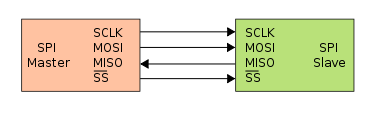
\includegraphics[scale=0.5]{figures/spi.png} 
\caption{SPI}
\end{center}
\vspace{-20pt}
\end{figure}\\
\textbf{SPI} hat 3 gemeinsame Leitungen und eine individuelle pro Slave, hier darf es nur einen Master geben, der das Clock-Signal an SCLK erzeugt. Mit der CS-Leitung kann der Master einen Slave auswählen, wird die jeweilige CS-Leitungen gegen Masse gezogen, so ist dieser Slave aktiv und wartet an MOSI auf Input und legt selbst seine Daten im Takt von SCLK auf MISO. Es wird dabei ein Byte vom Master an den Slave und ein anderes Byte vom Slave an den Master gesendet. \\
Mit jeder Taktperiode wird ein Bit übertragen, es sind also normalerweise 8 Taktzyklen notwendig für die vollständige Übertragung eines Bytes notwendig. 
\pagebreak

\section*{Aufgabe 4}


\begin{framed}
\textbf{ZigBee}\\
Was genau ist ZigBee und worin liegen die Unterschiede zu Bluetooth? ZigBee unterstützt den sogenannten "Beacon Mode". Worum genau handelt es sich dabei und was ist ein Beacon? Wie funktioniert die Übertragung im Beacon Mode? Geben Sie ein Beispiel dazu an?
\end{framed}

\pagebreak

\section*{Aufgabe 5}


\begin{framed}
\textbf{Schaltnetzwerke}\\
Zeigen Sie wie der Unterschied der Komplexität (Anzahl nötiger Schaltelemente) zwischen einer Corssbar und einer mehrstufigen Butterfly-Schaltnetzwerk zustande kommt.
Zur Erinnerung: Ein Crossbar-Switch hat Komplexität $O(n^2)$ im Vergleich zu einem Butterfly-Netzwerk $O(nlog(n)$, um $n$ Knoten miteinander zu verbinden. 
\end{framed}

\pagebreak

\section*{Aufgabe 6}


\begin{framed}
\textbf{CAN Bus}\\
Machen Sie sich mit dem Aufbau eines CAN Daten-Frames vertraut und erarbeiten Sie eine Formel zur Bestimmung der maximalen Netto-Datenrate $R(D,E,p)$ für die Nutzdaten in Abhängigkeit von DLC $D \in \{0,8\}$ byte, Extenden bit $E \in \{0,1\}$ und Busgeschwindigkeit in $p$ in bit/s. Geben Sie anschließend eine Formel zur Bestimmung des zugehörigen Protokoll-Overheads $\rho (D,E)$ an. \\
Bestimmen Sie $R(8,1,500000),R(8,0,500000)$ sowie alle möglichen Werte für $\rho$. \\
Wie muss die Formel für $R$ hinsichtlich der zu erwartenden Netto-Datenrate $R_{exp}(D,E,\rho, \alpha)$ verändert werden, wenn mit einer Paketfehlerwahrscheinlichkeit $\alpha \in [0,1]$ zu rechnen ist, die jeweils den Neuversand des kompletten betroffenen Daten-Frames erfordert? 
\end{framed}



   
   
\end{document}